\chapter{Related Work}
\label{chap:rw}

In this chapter, we would like to make the reader familiar with the variety of tools, which one can
use to analyze and visualize Linked Data. We will naturally compare these tools with
Payola, since in the past we participated on the proposal and development of this system.
Since the goal of this thesis is to propose and implement a system based on the Data Cube Vocabulary
standard we will, at first, focus on tools with the data cube support. 

We will provide a well--arranged table in order to present a quick overview of
what related tools are available at the time of writing this thesis and what are those 
tools capable of. Before we come up with the table let us mention, which
features are examined and why.

The main goal of this thesis is to deliver a prototype of a system, which will map 
arbitrary RDF data to a form compliant with the Data cube Vocabulary. Based on 
this fact, one of the criteria is an ability to \emph{convert arbitrary data 
into a form of cubes}. Another difference lies in a format of \emph{input data} of the
mapping process. There are tools working with relational (R), Linked Data (LD) or
arbitrary format (A).

The main benefit of implementing such a feature into Payola is that it becomes a 
part of an ecosystem. First of all, we have the user make an analysis over an~arbitrary
dataset (or, while using more than one data source even more than one dataset)
and then map it into the Data Cube Vocabulary standard. That also means that one is able
to analyze the data, interconnect them, filter them and enrich entities with more properties
while utilizing the principles of Linked Data before the mapping is made. Moreover, the statistical
dataset could be the result of an analysis. A new statistical dataset may originate from performing
such an analysis. On the other hand, many of the existing 
tools provide a way of converting a rather static dataset. Let's imagine a situation when a 
user has a database of statistical facts. While using a tool, they can 
convert the database into a set of triples according to the Data Cube 
Vocabulary format. When it is done they are able to apply Linked Data principles
on such a dataset. It might be a bit cumbersome to make the same analysis similar to
the previous case after the mapping is done. As the two use cases are dissimilar in process 
we will learn whether the existing tools make the user able to analyze datasets or \emph{create new ones}.

A part of the Payola ecosystem is also based on a fact that Payola is a web 
application with a \emph{sharing option}. A user is able to make an analysis (an
analytical algorithm or an analytical pipeline) and share it with other users. This applies also to 
analytical plugins, ontologies, etc. That is why we will differentiate between the following
application types --- desktop (D) and web (W). We will also want to 
know if it is possible to share \emph{within the application}.

There are also tools, which make the user capable of \emph{developing a custom vocabulary 
definition} (DCV data structure definition) based on the metadata of the input data.
This feature will be also covered in the overview.

While Payola is a platform for analysing and visualising data, we will also 
focus on the latter. First of all, it interests us whether 
an~examined tool makes the user able to \emph{prepare a visualization} . While keeping 
in mind the main principles presented in ~\cite{mantra} we will also discover 
which of these tools provide \emph{faceted browsing}.

What is also important to know is how a tool behaves while converting a rather 
\emph{large dataset}. We will not benchmark the tools but we will make a conclusion based 
on information available in corresponding papers since the authors usually make 
this very clear.


\begin{tabularx}{\textwidth}{ |r|C|C|C|X|X|X|X|X|X|X|X| }
  \hline
      \begin{sideways}Tool\end{sideways} & 
      \centering\begin{sideways}Cube support\end{sideways} &
      \centering\begin{sideways}Cube mapping\end{sideways} &
      \centering\begin{sideways}Mapping input\end{sideways} &
      \centering\begin{sideways}Analysing\end{sideways} &
      \centering\begin{sideways}Create datasets\end{sideways} &
      \centering\begin{sideways}Application type\end{sideways} &
      \centering\begin{sideways}Sharing\end{sideways} &
      \centering\begin{sideways}Custom vocabulary\end{sideways} &
      \centering\begin{sideways}Visualize\end{sideways} &
      \centering\begin{sideways}Faceted browsing\end{sideways} &
      \begin{sideways}Large datasets\end{sideways}\\ \hline
  \hline
  Payola                   & Y & Y & LD & Y & Y & W & Y & N & Y & N & N \\ \hline
  OLAP2DataCube    & Y & Y & R  & N & N & W & N & Y & Y & Y & Y \\ \hline
  Tabels                   & Y & Y & A  & N & Y & W & N & Y & Y & Y & Y \\ \hline
  CubeViz                & Y & N & -  & N & N & W & Y & - & Y & Y & Y \\ \hline \hline 
  
  Geo Globe             & N & - & - & N & - & W & N & - & Y & Y & N \\ \hline
  Visualbox              & N & - & - & N & - & W & Y & - & Y & N & Y \\ \hline
  ViDaX                    & N & - & - & N & - & D & N & - & Y & Y & Y \\ \hline
  LodVis                   & N & - & - & Y & - & W & N & - & Y & Y & Y \\ \hline
  Rhizomer              & N & - & - & N & - & W & N & - & N & Y & N \\ \hline
  Sgvizler                 & N & - & - & N & - & W & Y & - & Y & N & N \\ \hline
  Exhibit                  & N & - & - & N & - & W & Y & - & Y & Y & * \\ \hline
  Explorator             & N & - & - & N & - & W & N & - & Y & Y & Y \\ \hline
  Tabulator              & N & - & - & Y & - & W & N & - & Y & N & Y \\ \hline
\end{tabularx}

\section{OLAP2DataCube}
\label{olap2dc}
While comparing this tool we also rely on information presented by its authors in 
~\cite{ontowiki-paper}. The OLAP2DataCube tool is in fact a plugin for a well--known 
platform, the OntoWiki, which serves as an ontological knowledge base enabling
the~user to visualize and edit facts in the knowledge base in a specific way
while utilizing the principles of Linked Data.

The idea behind this tool is the closest to what we aim to achieve in this thesis.
In spite of this, it does something a bit different. It is designed to convert a 
whole relational database containing statistical data into a form of Data Cube 
Vocabulary. This also presents one of the biggest dissimilarities between the OLAP2DataCube and 
what we are about to propose --- the source is not in the RDF format.

The reason why this plugin was introduced was the need to convert a large 
dataset of statistical Brazilian government data into the Linked Data standard.
While doing that the authors wanted to build up on existing metadata standards, 
such as SDMX and therefore on Data Cube Vocabulary. This could provide the idea of 
what this tool does. It takes a dataset from a relational database and produces 
another dataset compliant with the Data Cube Vocabulary.

It could be advantageous to borrow principles of the relational databases world and have them
fit perfectly into the world of Linked Data. Tables in the relational database 
are organized into a shape of a star or a snowflake as described in Section~\ref{sec:datacube}.
Moreover, they are interconnected through defined foreign keys,
which can have the same semantics as edges in the directed RDF graph.
On the other hand, what is completely missing is any kind of structured
metadata. That is what the plugin needs to obtain from the user while the user
is required to give the data a precise meaning.

\begin{figure}
	\centering
	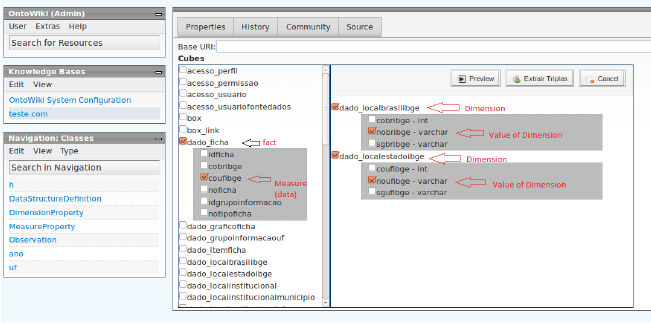
\includegraphics[width=140mm]{img/olapimport.png}
	\caption{OLAP2DataCube mapping specification example (taken from~\cite{olap2dc-paper})}
	\label{fig:olap2dc-screen}
\end{figure}


That is why the authors introduced some steps where the user is asked to 
do the following:
\begin{itemize}
  \item Select the fact table.
  \item Select dimensions tables.
  \item Enter additional metadata --- units, description, etc. or point to a 
  special dimension table containing the metadata.
\end{itemize}

The whole process of dataset conversion from relational database into Data Cube Vocabulary
(the authors call it triplification) is then divided into the following steps:
\begin{itemize}
  \item \emph{Metadata extraction and Table categorization} (PKs and FKs analysis). The 
  tables are precategorized as dimension or fact tables based on the number and 
  direction of FKs.
  \item \emph{Cube definition} done by the user as described in the previous paragraph.
  \item \emph{Mapping}. The relational database is converted into a Data Cube 
  Vocabulary compliant dataset while executing a set of SQL queries assembled 
  based on the previous steps.
\end{itemize}

As a matter of fact, this process has two different outcomes. A converted 
dataset itself and a definition of dimensions. This varies a lot from what 
we would like to achieve. We are about to propose a system, which will convert a 
dataset in order to comply with an already existing datastructure definition.

The authors have proven the system qualities by converting a dataset of Brasilian government data
into more than 31M triples, which is quite a large dataset. The faceted browsing
capability fully depends on the OntoWiki platform features.

\section{Tabels}
Tabels~\cite{tables-paper} is quite an interesting tool, which enables the user to 
convert arbitrary data into the Data Cube Vocabulary compliant format. 
Moreover, it allows the user to interconnect the data with its existing RDF 
representation, if available.

The most interesting feature of the tool is that it supports a large variety of 
input types. The user can pass a URL of an arbitrary website or upload a file 
in many supported formats. The application then generates an 
automated script, which converts the source document from the input format 
into the RDF while utilizing the Data Cube Vocabulary standard.

Let us imagine a case of converting a webpage. The tool parses the source code of the webpage and 
finds tables contained in the body of the page. Those are converted into a simple
RDF dataset. The same is done not only in the case of a webpage, but also in a case
of other specific supported file formats. To achieve that a specific algorithm is used to extract
the data from the file into a RDF graph. After this step is complete, the tool generates a DCV
datastructure definition in respect to the~kind of data found in the input dataset.
Also, an automatic conversion script, which the user can later execute in order to triplificate
the input data, is generated.

The script is written in a custom DSL (an example in Figure~\ref{fig:tabels}) which,
with its structure, resembles the well--known
transformation language XQuery. Although the script makes its job, the 
user may need to edit the script to improve the behaviour. That is one of the 
most problematic features of this tool. The user needs to have a heavy programmatic 
background in order to be able to use the advantages of all of the offered features. 
Even when binding the data in the input dataset with entities in an existing RDF 
dataset, the user needs to alter the generated script and specify, which field 
to bind and, of course, how.

\begin{figure}
	\centering
	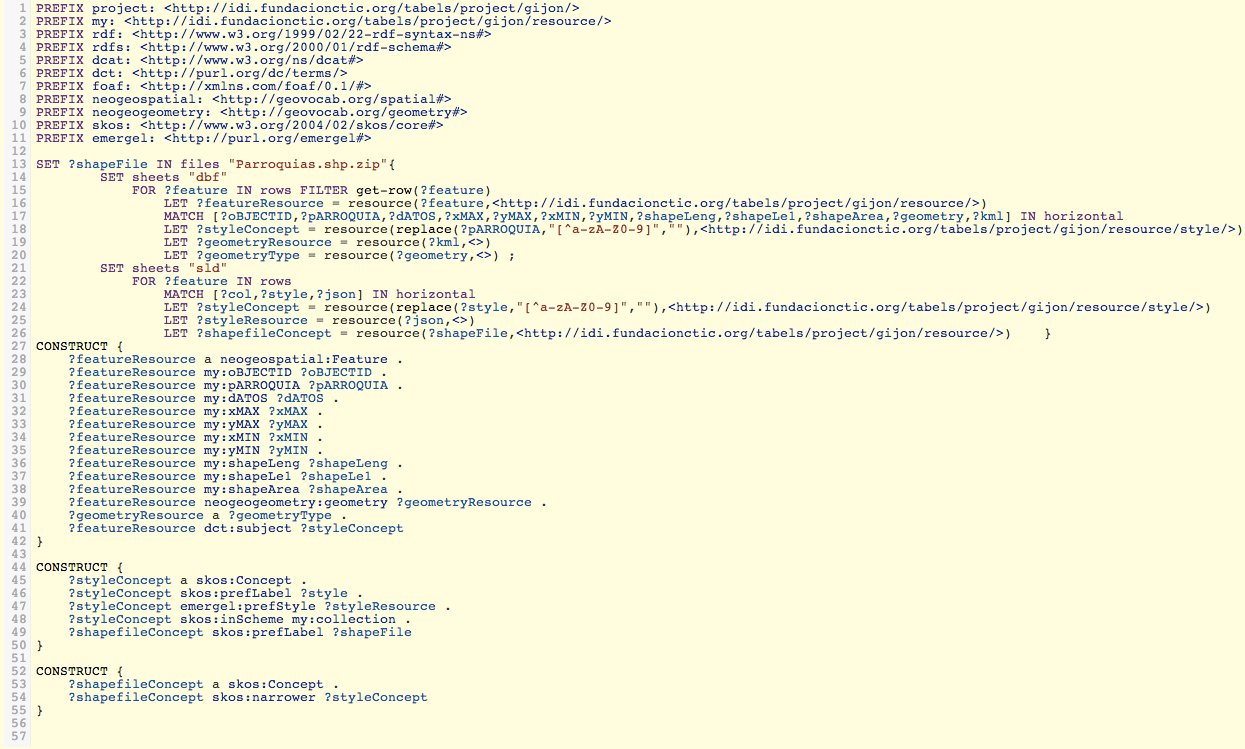
\includegraphics[width=140mm]{img/tabels.png}
	\caption{Tabels DSL example (script taken from examples repository~\cite{tabels-web})}
	\label{fig:tabels}
\end{figure}

On the other hand, the tool provides a unique form of making the user's own Data Cube 
Vocabulary dataset based on their statistical data in common file formats such as 
CSV, XLS, PX, KML and formats published by rather large institutions like Eurostat. 
The application is therefore able to visualize data in charts as well as on map 
in case of geospatial data.

Moreover, the tool also supports RDF as an input format, which makes it a 
competitor of the system we are about to propose. That is why we wanted
to examine this tool a bit more in the manner of processing different RDF 
datasets. Despite the fact that the tool should be able to process RDF 
datasets, it produced an empty conversion script even on DCV datasets downloaded 
from the tool itself. Therefore, the only form of converting the input file into 
the~DCV compliant dataset was to write the whole script manually, while 
specifying a set of SPARQL construct statements. That is, in fact, a default 
behaviour of any available SPARQL endpoint, which enables it to execute a SPARQL 
query on datasets.

\section{CubeViz}
\label{cubeviz}
The CubeViz tool has been developed by the AKSW~\cite{aksw} group
in the scope of the LOD2,
a~large--scale project co--funded by European Commission that is
focused on integrating and syndicating Linked Data with existing applications.

The motivation behind this tool was to bring a better user--experience into a 
large--scale application, developed by this group, called the \emph{Open Data Portal of 
European Commision}. While utilizing the Data Cube Vocabulary standard, they 
prepared a library of 5700 visualized statistical datasets.

\begin{sloppypar}
As well as the OLAP2DataCube tool, the CubeViz is also based on~the~\mbox{OntoWiki}~\cite{ontowiki}
application. In fact, it adds another layer to the 
technology stack and provides a way of exploring and discovering statistical 
data in a faceted browser. The GUI is made with common technologies like PHP,
HTML and JavaScript. They used the HighCharts~\cite{highcharts} library in
order to provide data visualization (an example can be seen in Figure~\ref{fig:cubeviz}).
\end{sloppypar}

\begin{figure}
	\centering
	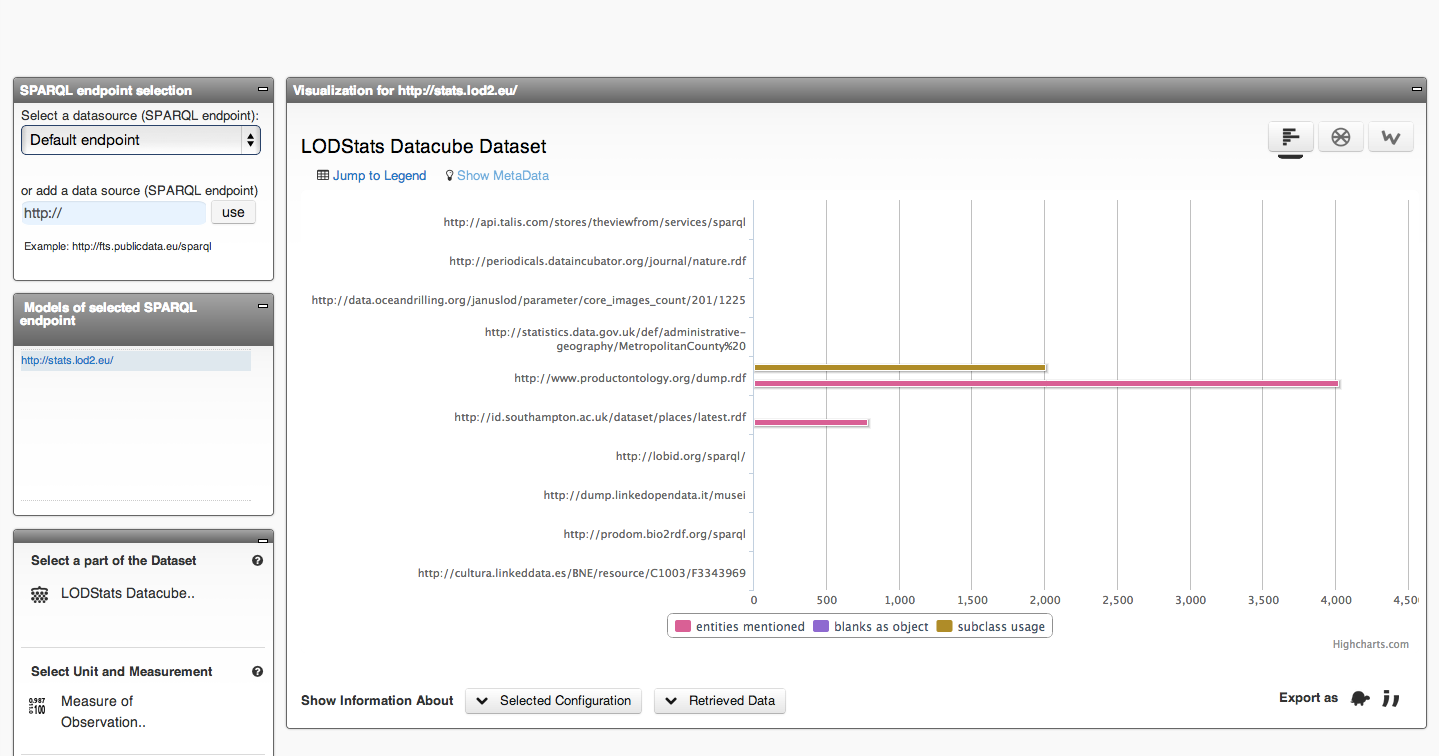
\includegraphics[width=140mm]{img/cubeviz.png}
	\caption{CubeViz visualization example}
	\label{fig:cubeviz}
\end{figure}

While utilizing the principles of Linked Data and Data Cube Vocabulary 
standard, the authors were able to come up with a really sophisticated faceted 
browser, which makes the user capable to filter data in detail based on the statistical 
semantics (DCV). The user is able to filter data based on each dimension, or to use the 
proper term, to slice the cube as needed. That gives us a generic tool, which 
compares any statistical data with the ability to learn more 
information while taking advantage of the entities Linked Data interconnection.

At the time of writing this thesis, the tool was limited to basic chart types
such as line, bar and pie chart (for datasets with one dimension). Those types 
were available also for the 2--dimensional datasets for which the polar 
chart is offered as well. More than two dimensions were not supported at all. In order to visualize 
multidimensional datasets one needs to slice it into a 2--or--less--dimensional one.
The tool also makes it able to publish dataset metadata.

An interesting feature of the faceted browser is that the user can 
generate a permalink in order to obtain a reference to the current visualization 
state. That makes it very easy for the user to share their visualization with the 
community.

\section{Visualbox}
Based on LODSPeaKr~\cite{lodspeakr}, a tool, which makes it easier to create Linked Data Websites 
and to publish RDF datasets, a visualization tool named Visualbox has been 
introduced. The motivation behind this was very similiar to those behind 
OLAP2DataCube, ViDaX or CubeViz. The author wanted to present a visual tool,
which would 
make it easy for the user to understand results of a data analysis.

The main argument is e.g. that a line chart is much more expressive and much easier
to understand than a table of data or some even more complicated data 
representation. Therefore, the author wanted to utilize existing visualization 
techniques people are used to intercept.

As a result of this effort, he presented a developer tool, which enables an easier preparation
of a visualization. One needs to know basic web development technologies 
in order to be able to use the tool. Specifically, the HTML language, the 
handlebars templating syntax and a concept of filters, which resembles the 
concept used in the JavaScript MVC framework AngularJS~\cite{angularjs}. One is however required
to posses the knowledge of the SPARQL in order to select data and prepare them for the 
visualization. An example of a SPARQL query and a visualization embed into a webpage can be seen
in Figure~\ref{visualbox-example}.

\begin{figure}
\scriptsize\begin{verbatim}

PREFIX conversion: <http://purl.org/twc/vocab/conversion/>
SELECT ?g sum( ?triples ) as ?estimated_triples
WHERE {
  GRAPH ?g  {
   ?g void:subset ?subdataset .
   ?subdataset conversion:num_triples ?triples .
  }
} 
GROUP BY ?g

{{models.logd.triples|GoogleVizColumnChart:"g,estimated_triples,width=1200"}}
\end{verbatim}\normalsize
\caption{Visualbox scripting examples}
\label{visualbox-example}
\end{figure}

On the other side, for those, who have this technological background the 
tool is really easy to use. By using a simple snippet, the developer is able to 
embed a chart visualization on the web.

The main benefit of this tool is that it brings a unified approach to 
visualising tabular data. Furthermore, it comes up with an informal standard of 
processing such data and visualising them. Based on the Google Charts visualization 
API, it allows the developer to visualize their data in basic charts 
as well as in a map if geospatial data are present. Although the features of the 
tool are mainly shown while visualising statistical data, the tool has no support for 
Data Cube Vocabulary.

\section{GeoGlobe}
The GeoGlobe mashup~\cite{geoglobe} is an example of a faceted browser for 
statistical data related to all the countries in the world. As the SPARQL 
query, visualization rules and more are hardcoded in this single--file 
demonstration, it serves us only as a great example of what could be the result of a
Data Cube Vocabulary dataset visualization.

The tool fires a XHR request to the server, which contains a SPARQL query. The 
query is executed in order to obtain data from a remote SPARQL endpoint. In 
fact, it uses some Data Cube Vocabulary constructs to filter the data. The data 
are sent back to the client in a form of a JSON string. The mashup then uses the 
D3~\cite{d3} visualization library in order to present the user with a D3 Geo 
visualization of the obtained data.

\begin{figure}
	\centering
	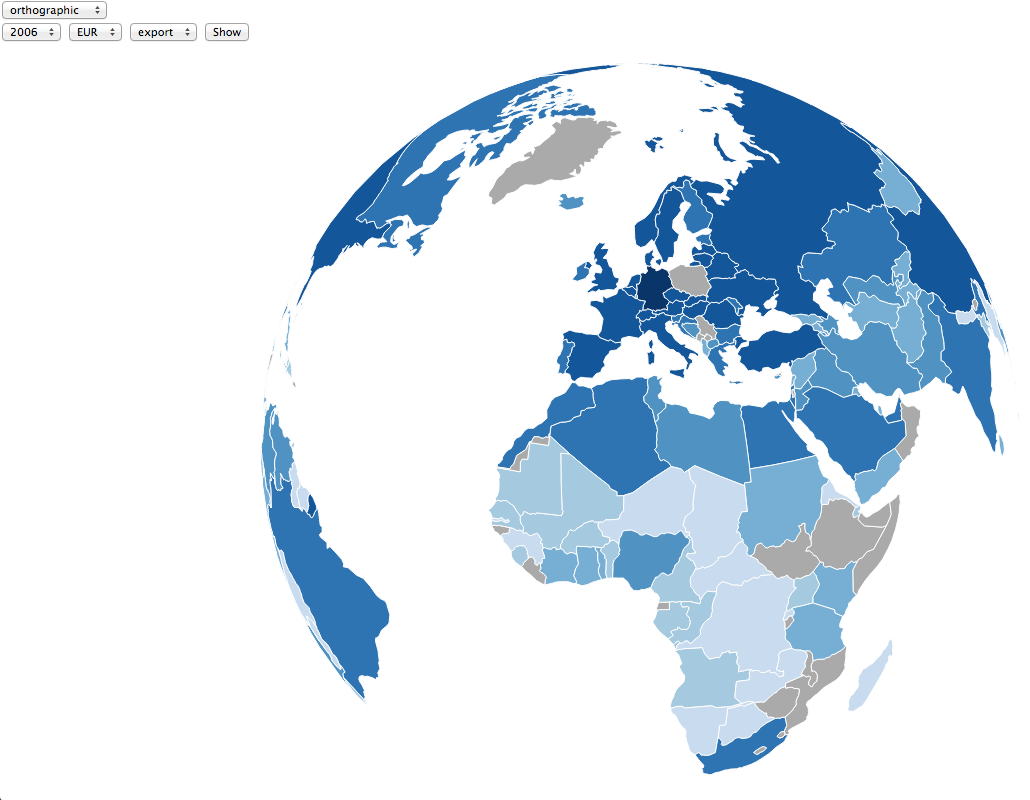
\includegraphics[width=140mm]{img/geoglobe.png}
	\caption{GeoGlobe visualization example}
	\label{fig:geoglobe}
\end{figure}


Simple GUI of the faceted browser changes the contents of the exectued SPARQL query. 
It decides how the original data cube is sliced to be visualized as the user 
wanted.

\section{ViDaX}
ViDaX is a desktop application written in the Java programming language. Based on the features
of the underlying visualization toolkit Prefuse~\cite{prefuse}, it manages to 
visualize RDF data in many ways. The toolkit is perfectly capable of 
visualising statistical data, but the application does not take advantage of the 
Data Cube Vocabulary standard.

Despite this, the application has some features related to statistical 
data. The visualization type is selected automatically based on the semantics of the 
visualized data. The application analyzes and normalizes the data selected by the user 
and extracts the types of the different properties. Those are consequently mapped to 
some basic supertypes such as Time, Location, etc. Based on the mapping,
the~tool offers a visualization template to the user.

As a result, the authors presented a tool capable of visualizing 
statistical data with appropriate visualization type without the need of using 
the~Data Cube Vocabulary standard. On the other hand, if the tool 
implemented the standard, the results could be even more reliable.

\section{Tabulator}
\label{sec:rw:tabulator}
Tabulator is a generic RDF browser and editor. The motivation behind this tool
is to provide a generic semantic browser with serendipitous re--use. The authors 
want to provide a form of finding more relevant datasets while exploring or 
publishing another datasets. 

The experimental version of the tool was, according to ~\cite{tabulator-paper}, 
developed completely as a client--side application for a web browser. Therefore, 
technologies like JavaScript, XHR, XML, RDF and SPARQL were utilized.

The tool offers two basic modes, exploration and analysis. In the exploration mode,
the~user starts to explore the Semantic Web by entering a URI of a resource. They 
are then presented with a tree view where each node represents a resource. 
By clicking the node, the user expands a subtree to obtain more information.
The tool implicitly follows links that may contain more relevant nodes.

In order to switch to the analysis mode, the user selects fields to define a 
pattern, which is then matched against the original graph. The tool executes a 
specific SPARQL query to find all occurrences of the selected pattern. The 
projection of this kind of analysis could be visualized in many different 
views such as a table, a timeline, a calendar and a map. The user can switch back to the 
exploration mode by double--clicking on an instance in the analysis view.

The most important feature of this tool is an implementation of a 
\emph{query--by--example} principle. By highlighting the properties in a tree view, the user 
unknowingly constructs a SPARQL query. As a 
result of such a process, the user may create a SPARQL query, which selects e.g., 
latitude and longitude. Dataset containing such properties (geospatial data)
is then visualized on a map. Although the tool is able to visualize statistical 
data, the Data Cube Vocabulary standard is not used.


\begin{figure}
	\centering
	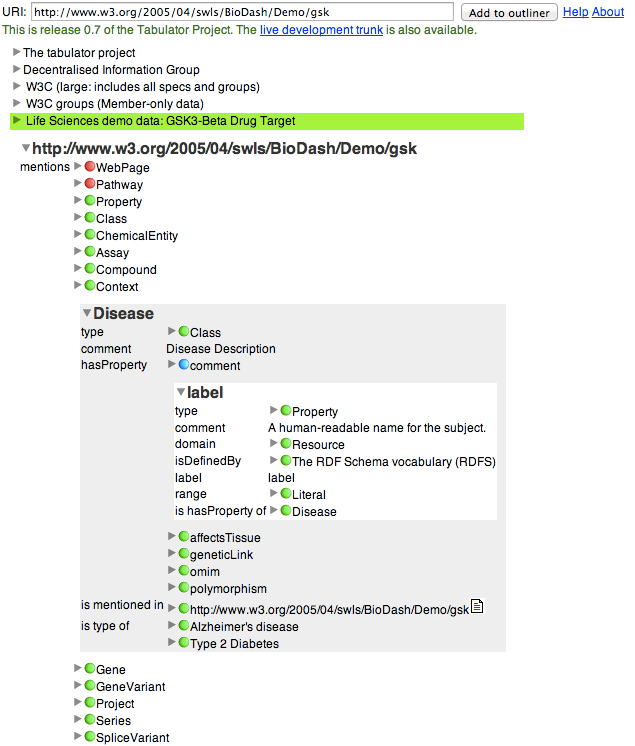
\includegraphics[width=100mm]{img/tabulator.png}
	\caption{Tabulator browsing mode example}
	\label{fig:tabulator}
\end{figure}


\section{Explorator}
\label{sec:rw:explorator}
The authors of the Explorator application had the same motivation as the authors 
of the Tabulator --- to come up with a tool that simplifies a dataset 
exploration. One can browse RDF datasets without a deep knowledge of the RDF standard.
In order to offer the~exploratory search~\cite{exploratory-search} feature, the authors also
utilized the query--by--example principle. Only simple so--called \emph{SPO SPARQL 
queries} (\texttt{SELECT \{ ?s ?p ?o \} WHERE \{ ?s ?p ?o \} }) are supported. Generally, the tool 
enables the user to specify a much simpler pattern than the Tabulator 
application. On the other hand, it offers a faceted browser, which generates 
those queries.

Unlike the Tabulator project, based on information presented in~\cite{explorator},
the~Explorator is not able to offer any advanced visualizations, such as a map or 
a chart. To speed up the application, the authors integrated a local SESAME~\cite{sesame} 
repository where dereferenced URIs are stored.

\section{Exhibit}
The MIT Simile project~\cite{mit-simile} has spent a more than a decade
developing and experimenting with software tools for Web--based data publishing.
As a result of the whole process a new tool, Exhibit, was introduced.

Exhibit is a JavaScript library, which produces embeddable widgets. A developer can
easily embed a visualization of a RDF dataset in an arbitrary web page. The idea behind 
the~tool is very similar to the idea behind the Visualbox project. After a quick 
examination, the use of the tool is no more complicated compared to the 
Visualbox despite the fact that the manual suggests so. As an example of a 
visualization, we can mention timeline, lenses and maps. Again, the tool is able 
to visualize data, which could be considered statistical, but it lacks the 
support of the Data Cube Vocabulary standard.

The tool became very popular for its rather easy--to--use 
approach of publishing visualizations. The very first version of the software
was introduced while completely ignoring the problem of large datasets.
Since it runs in a web browser, it needs to have the visualized data
fitted into the memory of the client 
computer. That is why U.S. Library of Congress initially funded the project to 
make its authors solve the scaling problem.

According to the information in~\cite{exhibit}
the~last version of the software supports $1000$ times more items in the
dataset ($100 000$ vs. $1000$) and up to $20 000$ properties in the faceted browser. 
The user is able to share views on the data after applying filters of the 
faceted browser. 

\section{Sgvizler}
The Sgvizler project is, as the name suggests, focused on data visualization. 
It is a JavaScript library, which parses an HTML source and finds specific 
element attributes. It fills matched elements with a data visualization based on 
the rules specified in the element attributes.

The developer is required to specify a SPARQL query as one of those attributes. The 
query is executed against a defined SPARQL endpoint. By setting an attribute of
the~placeholder element, the user also specifies the type of visualization, which 
should be applied on results of the SPARQL query execution.

As well as the aforementioned tools, Sgvizler is also capable of visualising statistical data, 
but the Data Cube Vocabulary standard is not used in any way. For instance, in 
the~case of a map visualization, the library expects the query to return a table 
with a location name in the first column and a measurement value in the second 
one. It does not really take advantage of the semantical properties in the 
dataset.

\section{Rhizomer}
Another tool focused on faceted browsing is Rhizomer. It is a web application 
offering quite an interesting feature, which partially fits into the LDVM 
concept. Based on data filtered by the faceted browser, the user is hinted about
which visualizers are available. Moreover, 
it indicates how many entities of the current view will be displayed after 
switching to the more advanced browsing mode.

As usually, those advanced modes are a timeline, a map and a chart visualization . As 
in the previous cases, the tool also works with datasets that could be 
classified as statistical, but it does not comply with the DCV standard. On the 
other hand, it relies on semantics of the data and autodetects properties, 
which can have a dimensional meaning, e.g. latitude and longitude for geospatial data.

\section{LODStats}
The authors of the LODStats project suggested that a major 
problem while working with data on the Web is to get a clear picture of the 
structure of a dataset. They also introduced a term \emph{external coherence},
which explaines how well the resources of the examined dataset are connected with 
other resources, generally speaking, how the dataset is interconnected with 
other datasets.

In order to solve the problem, they have introduced the LODStats project, an 
extensible framework optimized to work on a rather large datasets. Its purpose 
is to compute statistics on the given datasets. The tool is integrated with the 
CKAN~\cite{ckan} dataset metadata registry (The Data Hub~\cite{thedatahub})
in order to cover the most known and 
most used datasets, therefore to offer statistics for a great part of the Data 
Web.

Since one can overview rather small datasets without any significant problem, 
the~biggest advantage of the LODStats tool lies in the ability to work fast with 
datasets containing millions of triples of RDF data. The authors took advantage 
of the presence of a SPARQL endpoint, which allows them to work with the datasets 
dynamically, without the need to load all those millions of triples into the 
memory.


\begin{figure}
	\centering
	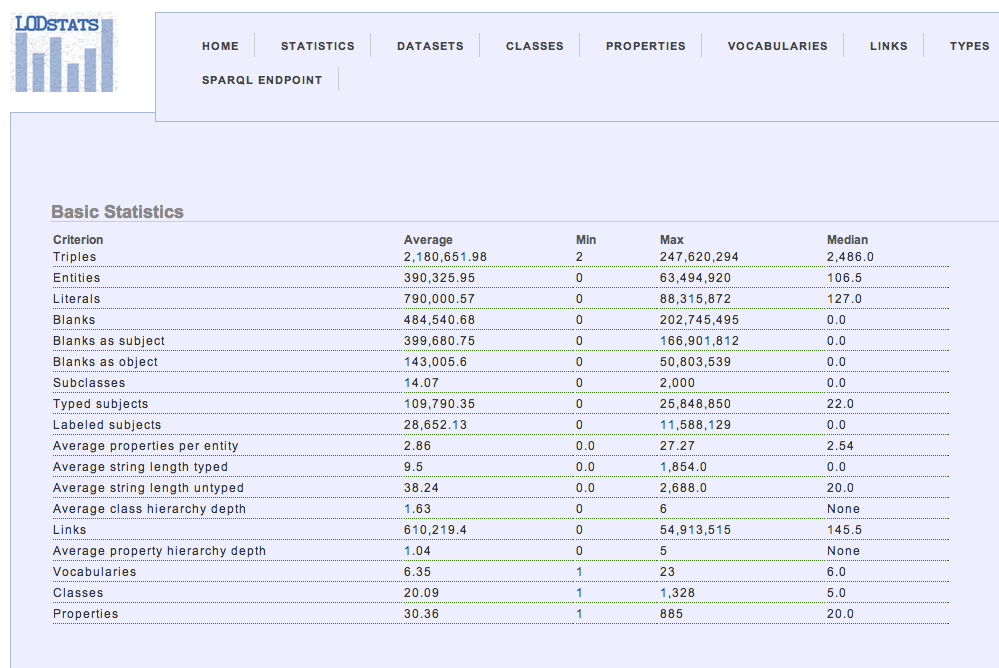
\includegraphics[width=140mm]{img/lodstats.png}
	\caption{LodStats statistics example}
	\label{fig:lodstats}
\end{figure}

The way of processing a dataset with a large amount of triples is an approach 
which Payola should definitely adopt in the future.

The authors of the tool implemented statistics that were defined by VoID~\cite{void}. Which 
means that 32 different statistics are computed while utilizing the following 
approaches:

\begin{itemize}
  \item \emph{Quality analysis} --- The problem of a dataset quality is tightly connected 
  to the form of the eventual data use. Therefore, a static analysis should 
  give us a general purpose measure (similar to Google's Page Rank) to determine the 
  quality very briefly, e.g. based on the number of outgoing and incoming 
  edges.
  
  \item \emph{Coverage analysis} --- The authors present two subtypes of 
  coverage - \emph{vertical} and \emph{horizontal}.  While the horizontal is 
  introduced to determine the size of the domain (how many resources are described),
  the vertical deals with the scale of details (how deeply the description goes).
  
  \item \emph{Privacy analysis} --- While analyzing what classes and properties 
  are used, the authors of the project try to determine if a dataset 
  might contain any personal information.
  
  \item \emph{Link target identification} --- According to the authors, less than 
  10 \% of entities on the Data Web are interlinked. This technique 
  should help the user determine what dataset should the examined one be 
  connected with.
\end{itemize}

Since the authors have focused on performance and declared to develop a 
tool with a smaller memory footprint and better scalability, it 
would be really useful to integrate such a tool with the Payola tool.
The integration would give the Payola user the opportunity to get familiar with the 
chosen dataset before analyzing it. In fact, as a circumstantial goal of this 
thesis, we will integrate the tool (on HTTP communication basis) with the previously mentioned 
LODvisualization application, the illustration of the concept introduced 
in~\cite{ldvm}. Integrating Payola with the LODStats analyzer should be also 
possible since the source code of both tools is available on GitHub~\cite{github-payola} 
~\cite{github-lodstats}, but that is not a part of this thesis.

The authors made the tool to examine a given dataset in two ways, to examine 
the~\emph{schema-level characteristics} and \emph{data--level characteristics}. 
The former describes the characteristics of an entity in the context of the used 
schema fragments (e.g. depth in a tree where hierarchical ontologies are used). 
The latter then describes the characteristics related directly to the values 
appearing in the dataset (such as minimum, maximum values, average values, entities equality, 
etc.). An example of computed statistics can be seen in 
Figure~\ref{fig:lodstats}.

One will learn very quickly that Payola and LODStats are focused each 
on something completely different, but can complement each other very well. The Payola 
tool should definitely learn from the statement--stream--based approach in order 
to handle larger datasets better. The authors of the tool also published
some statistics~\cite{lodstats} gathered while integrating with the CKAN database, which is a 
great source of information when trying to get the idea of how an average dataset 
could look like. 

\section{Yahoo Pipes, DERI pipes}
There are many analytical tools for processing RDF data. We would like to 
compare the Payola tool with the most important of them and provide the most significant 
differences. When deciding how the Payola tool should work, we came 
across an existing tool --- Yahoo 
Pipes~\cite{yahoo-pipes}. Providing an interactive 
editor, it allows the user to construct his own analytical \emph{pipe}, 
which, in fact, corresponds with the term \emph{analyser} (as defined in LDVM~\cite{ldvm}).
The only exception is that the various offered data sources are
providing plain XML data (they are not in the RDF format).
The tool does not offer the same level of analyzing data.
It would be very hard to simulate SPARQL with tools like XPath.

That is how we came up with the idea of \emph{analyses} concept for Payola. 
We offered a basic editor, which enables the user to build his own analysis
(also called an \emph{analytical pipeline}).
 
On purpose we made the editor with a rather restrictive behavior in order to 
avoid creating invalid or incomplete analyses. The user is able to insert new 
plugins into an existing analysis (analytical pipeline) only by connecting it to an output of another 
one. Since we are analyzing RDF data, the basic set of plugins is strongly 
related to the capabilities of the SPARQL.

After a while, we came across the DERI Pipes 
project~\cite{deri-pipes}, which is also inspired by the Yahoo 
Pipes project and is focused on processing RDF data. The editor is distributed 
in a form of a Java JAR package, therefore, one should be able to integrate it in another
Java--based software rather easily.

Unlike Payola, it contains some basic text operators, which even enables the user  
to construct the URL that is used as a parameter of the RDF data fetcher. This 
is also the biggest difference between DERI Pipes and Payola: Payola lets 
you work only with RDF data which is the reason why plugin parameters (with basic data types string,
boolean, integer and float) could not be computed in the process and are 
statically given by the user when defining an analytical pipeline.

\begin{figure}
	\centering
	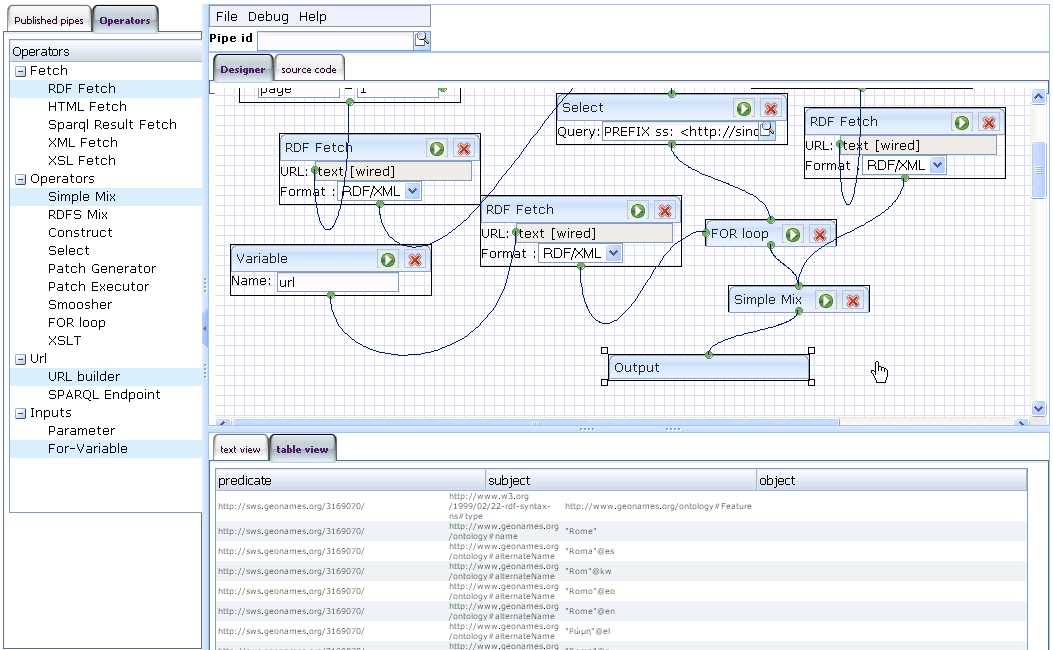
\includegraphics[width=140mm]{img/deri.png}
	\caption{Deri Pipes example as shown in an instruction videocast~\cite{deri-screen-source}}
	\label{fig:deri}
\end{figure}

The DERI Pipes tool offers some of the operators provided also by Payola. Some 
of them require the user to know the SPARQL in order to fill in the 
parameters, e.g. the \texttt{SELECT} operator. One may also apply XSLT 
transformation operators and use \texttt{FOR} loops. It also enables the user to use more datatypes as an input 
of a pipe, for instance a classic HTML document.

\section{Payola visualization model vs. LDVM}
The primal reason of the Payola tool implementation was to prove some basic concepts:

\begin{itemize}
\item Generic Linked Data analysis with a web application.
\item Generic visualization of analyses results.
\item All--in--one (read, share, analyze, visualize) Linked Data tool.
\end{itemize}

As the original intent of the tool was not to implement any specific existing visualization model,
the~system has been created with its own internal visualization pipeline architecture. Let us compare such
an~architecture with the model proposed in~\cite{ldvm}. For an easier orientation, let us name the Payola visualization 
model as a \emph{Payola model}. The model proposed in~\cite{ldvm} is named \emph{LDVM}. We will describe the Payola
model while utilizing the terms used in~\cite{ldvm}. Moreover, we will also explain
the~differences between the LDVM and the Payola model.

The Payola system is able to visualize all kinds of RDF data. It retrieves them from different
types of RDF storages. Since it is not currently important, suffice it to say that it just fetches
arbitrary RDF raw data. It uses SPARQL \texttt{CONSTRUCT} queries to retrieve those data from
the~given sources in order to work with graphs.

After the dataset is fetched, it is processed by an \emph{analyzer}. This could be a set of any kind
of transformations or operations. The most common case is running a SPARQL query
on the input graph. The only invariant is that the analyzer retrieves a RDF graph
representation and its output is also a RDF graph representation (regardless of a concrete
implementation). This is the phase described in~\cite{ldvm} as \emph{Data transformation}.
Naturally, the product of such an operation is a result of the analysis, which is called an
\emph{Analytical abstraction} in~\cite{ldvm}.

Since Payola is a web application, which delegates rendering the view to the client--side
of the application, the result of an analysis is transformed into a simplified format for a \emph{visualizer}.
At first, the result, which is an RDF format representation, is serialized to a custom \texttt{JSON} string
that is transferred to the client--side. The string is then deserialized to an internal visualizer
representation. In fact, this procedure is similar to one called \emph{visualization transformation}
in~\cite{ldvm}. The product is the \emph{visual abstraction}~\cite{ldvm}.

When the visualizer has all the data it needs, it maps the visualization abstraction to a visual
representation, or, as described in~\cite{ldvm}, to a View. Actually, the process of mapping in~\cite{ldvm}
described as Visual mapping transformation is just traversing the retrieved data and interpreting
them in a visual form (regardless of the concrete form).

As one can see, the Payola model and the LDVM are very similar. In fact, the Payola pipeline
architecture corresponds with the proposed LDVM with some minor exceptions. Some of them
originate from the fact that the Payola model is the result of an implementation
based on concrete technologies. That is why some additional constraints (especially
the~graph invariant) are added.

Another exceptions issue from the modularity of the Payola system. The system was designed
to provide a platform, which also means that the developer is able to build his own visualization 
plugins. This suggests as well that while serializing data into the JSON, the platform cannot perform
any data optimizations in order to preserve all available information. Let us remind the reader of
a~part of visualization transformation definition from~\cite{ldvm}:

\emph{The goal of this transformation is to condense the data into a displayable size and create
a~suitable data structure for particular visualizations.}

This operation may be repeated \emph{on--the--fly} in the visualization mapping transformation
phase by the concrete visualization plugin chosen by the application user. In fact, one can
say that the visualization transformation phase is duplicated and the pipeline contains two
stages of \emph{visual abstraction}. One can see an overview of the Payola 
visualization model in the fig.~\ref{fig:payola_model}.

\begin{figure}
	\centering
	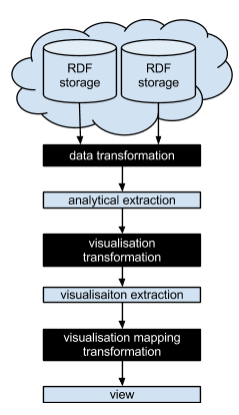
\includegraphics[width=100mm]{img/payola_model.png}
	\caption{Payola visualization model}
	\label{fig:payola_model}
\end{figure}

\subsubsection{LOD visualization}
To prove the concept of LDVM, one of the authors decided to come up with a tool 
based on the concept. The LOD visualization tool~\cite{lodvis} is oriented
to perform well on rather big datasets and 
provide their main characteristics in a reasonable time. Its main purpose is to 
enable to orient quickly in a given dataset. It provides several 
visualization types that help the user to understand the structure of the 
dataset.

That is also the most significant difference between the Payola tool and LOD 
visualization. The basic Payola analyzer and visualizer implementation provides 
deep details. It shows the whole dataset in the most possible detail. In fact, 
the~performance could become an issue on a rather large dataset.

Those two tools are actually complements. While working with a dataset one could 
start with the LOD visualization tool to get the overall picture of the dataset --- 
the~\emph{data coherence}. It will also help to get the idea of what is included in the 
dataset without making a specific query.

Payola comes in when one is familiar with the structure of the dataset. The user 
is now able to perform specific queries, analayze the dataset and attempt to make a 
visualization of the analysis result. Therefore, one of the minor tasks of this thesis
will be a simple integration of the LODvisualization tool into Payola.

\begin{figure}
	\centering
	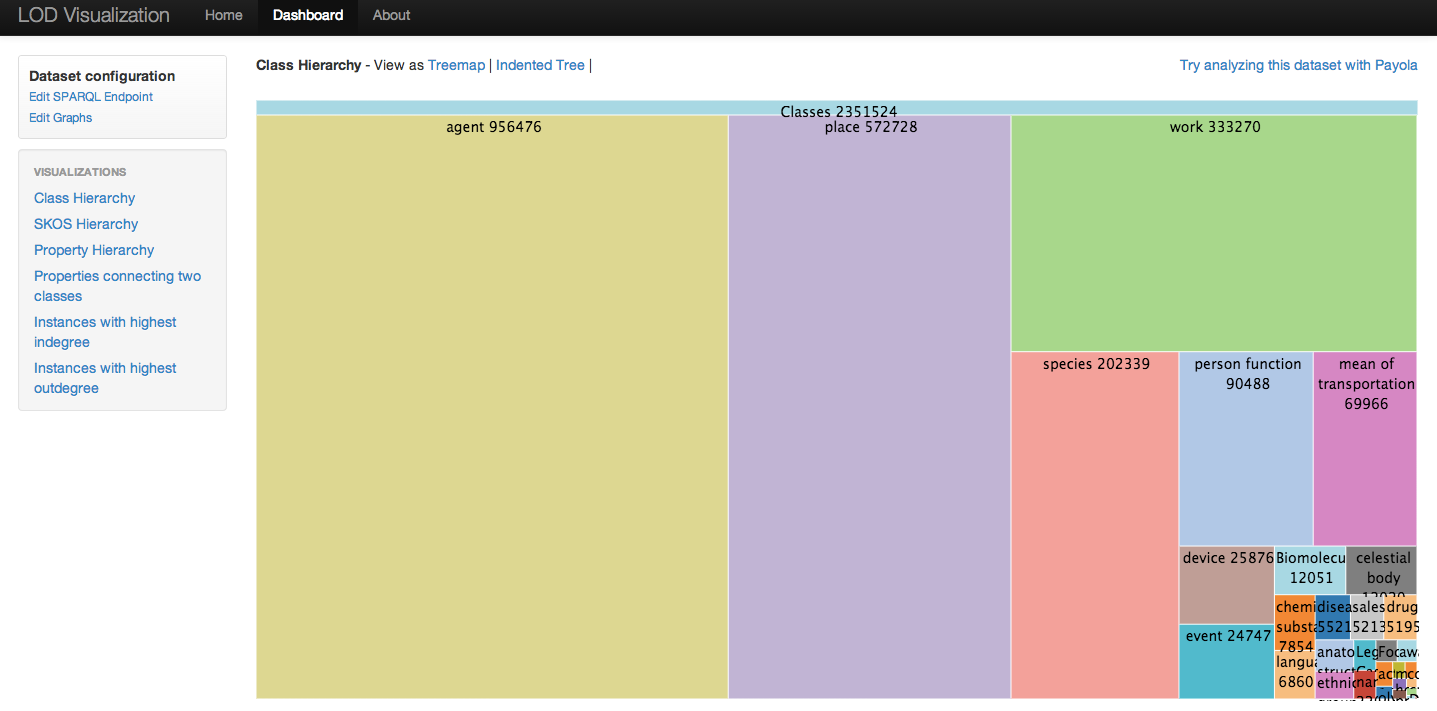
\includegraphics[width=140mm]{img/lodvis.png}
	\caption{LodVis visualization of DBPedia class hierarchy}
	\label{fig:lodvis}
\end{figure}

The user of the LOD visualization tool is able to utilize the following 
visualizations:

\begin{itemize}
\item Class hierarchy.
\item SKOS hierarchy.
\item Property hierarchy.
\item Properties connecting two classes.
\item Instances with the highest indegree.
\item Instances with the highest outdegree.
\end{itemize}

In a form of an interactive treemap or tree view, one 
can traverse through the tree that expresses the hierarchy of RDF classes used 
in the given dataset. One can also do the very same thing with properties. The 
user is also able to list all of the properties that are somehow (in both directions)
connecting any two classes from the dataset. When given a class, the tool is 
able to quickly find an instance of such a class, which is the most referenced
instance. It is also able to determine what instances have the largest amount of references
--- they have the highest amount of outgoing
edges.

\subsubsection{The extended version of LDVM}
Since the original paper was published on ISWC 2012 as a demo and a
work--in--progress, the model is being developed even while writing the text of 
this thesis. We will operate with the latest available version~\cite{ldvm2} and look 
at the new features of the proposed model. In fact, the latest version of the 
paper also covers an evaluation of RDF data visualization tools including 
Payola.

The most significant change came with introducing the concept of a \emph{visualisator 
reusability}. The authors talk about so--called~\emph{GVDTs} (Generic visualization Data Types).
That forces us to think about what types of visualizators we could need. That applies also to
one of the~core products of this thesis --- visualizators for multi--dimensional data.
One will probably repeatedly use a limited count of visualizers.

While Payola makes it possible to reuse a visualizer, it does not satisfy the 
requirements set down in the proposal~\cite{ldvm2}. The idea goes a little bit 
further, beyond the borders of a single application. Being integrated with the 
LOD cloud, it should be possible to query it with the characteristics of 
the~data we would like to visualize and get a list of visualizers 
available in the cloud and suitable for the task.

By reusing this concept, the same could be applied to analyzers and so--called 
\emph{transformers} designed to transform the results of an analysis 
into another form more suitable for a certain class of visualizers. 
That could include a process of gathering more useful data (e.g. to visualize 
some data on a map it is needed to enrich the dataset with a GPS locations).

The result is a dynamic pipeline architecture(\emph{LDVM Pipeline Instance}),
starting with an arbitrary 
dataset passed to some analyzer followed by a chosen transformer ending up with
visualising the result with one of the visualizers. As a result of applying the concept,
we would obtain something similar to dynamic 
registry of analyzers, visualizers and transformers.

To make the Payola tool 
compliant with this concept, we would need to introduce a module, which allows the user
to describe the analyzer (user--made analyses) and make the 
analyses more reusable. Currently, each analysis is tightly connected to the 
data sources it utilizes and those cannot be easily switched. That would, in 
fact, require massive changes in the analyses editor, which is not very 
user--friendly when it comes to editing an existing analysis.

The concept of transformers is completely missing in Payola since, as stated 
before, it is up to each visualizer to transform the passed data into a more 
suitable form, even enrich them with necessary information.

All the visualizers currently implemented in the Payola stack are fully 
reusable. But the tool lacks the feature to receive data from an external source 
and apply a visualizer on them. Or, from another point of view, there is no 
way of invoking the visualizer itself and specify where the data is and execute a 
visualization process.

All those missing features have one thing in common. Payola is missing 
an~API, which would be able to tell, which analyzers, transformers and 
visualizers are present in the current installation of the tool and provide a 
machine--readable description of such components. Moreover, it is missing a 
mechanism that will allow the user to run those components separately out of 
the~context of the Payola tool.

The authors call the above a \emph{compatibility} in the~\cite{ldvm2} and 
introduce a formalization that involves defining an \emph{input signature}.
In case of the basic Payola components, with an exception of one visualizer, the signatures
would be empty. This would effectively express the fact that they are designed to
visualize every dataset. The only exception is the \emph{Chart visualization},
which requires the data to have a specific pattern so it would be sufficient to sign it 
just with a SPARQL query. While speaking about analyses made by the user or more 
advanced visualizers, ontologies would also come in.

\section{Payola visualisator framework features}
Since there are generally many publications focused on data visualization (with no
connection to Linked Data), we would like to compare the recommended approaches to
the~implementation of visualizers embedded in Payola.

Ben Shneiderman in~\cite{mantra} introduces a term \emph{Visual lnformation--Seeking Mantra}.
He tries to define
what a good visualizer should provide to satisfy its user. He also puts those definitions into
a~context with some specific data formats, more particularly with multi--dimensional data,
which are related to the topic of Linked Data, moreover the Data Cubes metaformat. We try to
compare the specified list of features with those provided by Payola. We also want to explain,
why some of those features are missing or provided in another form.

The author states that every visualizer should have the following features:

\begin{itemize}
\item Overview.
\item Zoom.
\item Filter.
\item Details-on-demand.
\item Relationship view.
\item User actions history.
\item Sub-collections extractions.
\end{itemize}

Let us go through the list of the features and comment them gradually. All the visual plugins
embedded within Payola provides the \emph{Overview}. It is important to state
that it contains some limitations. Since Payola is a generic Linked Data visualization tool,
the~output of practically all of the plugins is a graph (network). It contains all of the vertices
included in the visualized dataset. Those are placed by a given algorithm on the screen,
but are not clustered. The result is that the user is (in most cases) able to see the whole
dataset on his screen. But the visualization could be a bit confusing since all the vertices
are present. The recommended adjustment would be to somehow simplify the initial view.

\begin{figure}
	\centering
	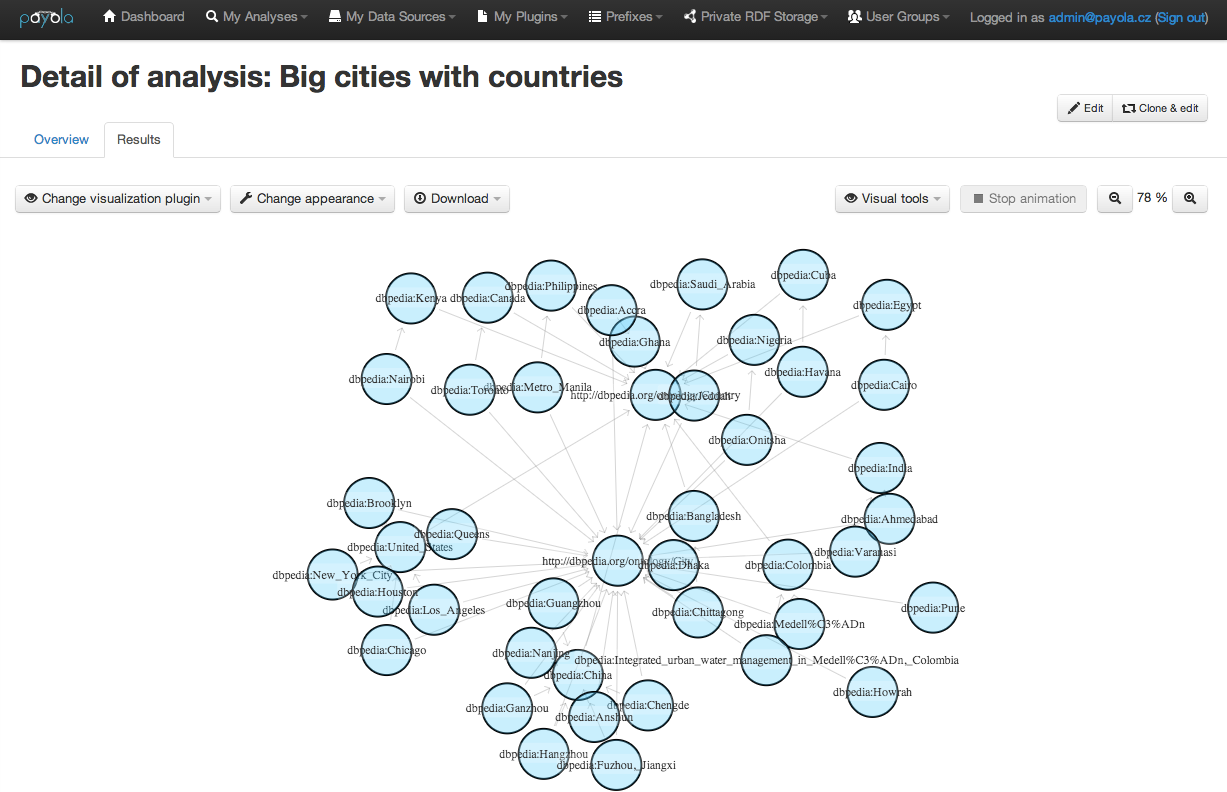
\includegraphics[width=140mm]{img/payola.png}
	\caption{Payola analysis result visualization}
	\label{fig:palyola-vis}
\end{figure}


The visualized graph might be dense one. Some of the used algorithms will create a graph, which
will have virtual clusters of vertices with a very little distance between them. In fact, some of those
vertices would be so close to one another that they would overlap. Therefore Payola enables the
user to \emph{zoom} in and regulate the virtual distance between vertices.

When speaking about the \emph{Details--on--demand} feature, we would like to distinguish
between two different
scenarios:

\begin{itemize}
\item Detailed information about a vertex.
\item More detailed relationship information.
\end{itemize}

To make the view more synoptic many of the embedded plugins extract the related literal
vertices and collapse them into a vertex meta information. E.g. the entity
\url{http://dbpedia.org/resource/Dhaka} has some properties - \texttt{label},
\texttt{populationDensity}, \texttt{populationTotal}.
Those are actually relations. Despite that fact, visualizers do not treat them
that way. They store this information in the memory and display it if and only if the user
interacts with the related vertex.

The most missing Payola feature is loading relationships on--demand. With the connection to the
problem
mentioned in the overview section of this chapter it would be more suitable, if the Payola system
would enable the user to view only significant vertices at first and only load details when needed.
This is also connected to the \emph{Sub--collections} extractions feature, which is partially available
in the analytical Payola module.

Since Payola visualizes Linked Data, it naturally visualizes the \emph{relations between the entities}.
The only feature, which is rather missing in comparison to the feature list from~\cite{mantra}, is
\emph{User actions history}.
There is only one component of Payola that make a user able to walk through 
history of actions and that is a SPARQL endpoint browser. It remembers the path 
that user creates while clicking through the dataset. The other visualizers 
however are not equipped with such a feature.

Payola does not fulfill the basic thought stated in~\cite{mantra}, since 
there is no visualization plugin that would enable the user to overview the 
examined data set via a specialized visualization such as a treemap 
in~\cite{lodvis}. What one gets after visualizing the results of an analysis is a 
detailed view, which is (in the case of graph visualizations) however zoomed out
to enable the user to see the whole dataset at once. Despite that fact, it 
contains representation of all the nodes in the data set and therefore breaks 
the~visual information seeking mantra.
